
\breaksection{External elements}\label{sec:quantification_external}

\subsection{Introduction}

\boxgreen{\textbf{External drivers}}{
        \textbf{Scenario elements}
        \begin{itemize}
          \item \textbf{Demographic change:} \\ population, median age, urbanisation, gender 
          \item \textbf{Economic growth:} \\ GDP
          \item \textbf{Renewable energy transition:} \\ energy mix
        \end{itemize}
        \textbf{Waste model parameters include:}
        \begin{itemize}
          \item \textbf{Put-on-market}
          \item \textbf{Composition}
        \end{itemize}
        \textbf{Recovery model parameters include:}
        \begin{itemize}
          \item \textbf{Recovery processes:} \\ market penetration of recovery technologies
          \item \textbf{Transfer coefficients:} \\ function of recovery technologies
          \item \textbf{Recovery system size:} \\ BAU - set by trends in BAU, CIR \& REC - defined by model outcomes within constraints
        \end{itemize}
        \textbf{Impact model parameters include:}
        \begin{itemize}
          \item \textbf{Foreground inventory:} \\ inputs and outputs of recovery system
          \item \textbf{Background inventory:}\\  energy mix, impact of primary production
        \end{itemize}
          }


In the FutuRaM project, scenario elements are categorised based on their influence and relevance to the secondary raw material (SRM) system. This categorization aids in refining the focus of the scenarios and ensuring they are relevant, manageable and useful.

Following the process detailed in \autoref{chapter:methodology}, several scenario elements were classified as "external" or "outside". 

The following "external" elements are incorporated into the scenarios as background information but are not directly modelled. They are assumed to be constant across the three scenarios, but change over time.

\begin{itemize}
    \item Demographic change 
    \item Economic growth  
    \item Renewable energy transition 
\end{itemize}

The following "outside" elements are not incorporated into the scenarios, but are considered important and will be explored in sensitivity analysis and optimisation.

\begin{itemize}
    \item Resource supply constraints 
    \item International trade and co-operation 
    \item Re-industrialisation of EU 
    \item Resistance to recovery projects ("NIMBY") 
\end{itemize}

These elements are detailed in \autoref{tab:elements-external}.

\begin{landscape}
\begin{table}[h!]
    \centering
    \small
    \caption{List of external scenario elements}\label{tab:elements-external}
    \begin{tabular}{|C{1.5cm}|L{6cm}|C{1.5cm}|C{1.5cm}|C{1.5cm}|C{1cm}|C{1cm}|C{1cm}|L{6cm}|}
      \hline
      \rowcolor{headerblue} % Applying the header color
      \textcolor{white}{\textbf{DOMAIN}} & \textcolor{white}{\textbf{ELEMENT}} & \textcolor{white}{\textbf{INTERNAL}} & \textcolor{white}{\textbf{EXTERNAL}} & \textcolor{white}{\textbf{OUTSIDE}} & \textcolor{white}{\textbf{BAU}} & \textcolor{white}{\textbf{REC}} & \textcolor{white}{\textbf{CIR}} & \textcolor{white}{\textbf{MODEL PARAMETERS AFFECTED}} \\
      \hline
      ECO & Progress toward renewable energy targets & & \checkmark & & - & - & - & composition, demand, waste generation, recovery impacts \\
      ECO & Economic growth & & \checkmark & & - & - & - & composition, demand, waste generation \\
      SOC & Population & & \checkmark & & - & - & - & demand, waste generation \\
      ECO & Primary vs. secondary raw material prices & & \checkmark & & \textasciitilde & \textasciitilde & \textasciitilde & considered in sensitivity analysis \\
      ECO & Energy prices & & \checkmark & & \textasciitilde & \textasciitilde & \textasciitilde & considered in sensitivity analysis \\
      ECO & Carbon price & & \checkmark & & \textasciitilde & \textasciitilde & \textasciitilde & considered in sensitivity analysis \\
      ENV & Resource supply constraints & & \checkmark & & \textasciitilde & \textasciitilde & \textasciitilde & considered in sensitivity analysis: \\
      ECO & International trade and co-operation (vs. autarky) & & & \checkmark & n/a & n/a & n/a & not model input (resource supply constraints is a proxy) \\
      ECO & Re-industrialisation of EU & & & \checkmark & n/a & n/a & n/a & not model input \\
      SOC & Resistance to recovery projects (NIMBY) & & & \checkmark & n/a & n/a & n/a & not model input (considered in UNFC assessments) \\
      \hline
    \end{tabular}
  \end{table}
\end{landscape}

\clearpage
\subsection{Summary}

\boxreview{This summary will be compiled once the individual waste stream sections for each parameter are complete.}

\subsubsection{Demographic change}


\subsubsubsection{Independent variables}
    \begin{itemize}
        \item Population
        \item Median age
        \item Urbanisation
    \end{itemize}
    
\subsubsubsection{Dependent variables}
    \begin{itemize}
        \item Demand
        \item Waste generation
        \item Waste composition
    \end{itemize}

\subsubsection{Economic growth}


\subsubsubsection{Independent variables}
    \begin{itemize}
        \item GDP growth
    \end{itemize}
    
\subsubsubsection{Dependent variables}
    \begin{itemize}
        \item Demand
        \item Waste generation
        \item Waste composition
    \end{itemize}

\subsubsection{Renewable energy transition}


\subsubsubsection{Independent variables}
    \begin{itemize}
        \item Energy mix
    \end{itemize}
    
\subsubsubsection{Dependent variables}
    \begin{itemize}
        \item Demand
        \item Waste generation
        \item Waste composition
        \item Recovery impacts
    \end{itemize}

\subsubsection{Resource supply constraints}

\boxnote{This element is not forecast or modelled directly, but is considered in sensitivity analysis and optimisation. \\ Supply constraint is independent of its cause (e.g. resource depletion, political instability), thus, it can act as a proxy for other elements such as international trade and co-operation.}

\subsubsubsection{Independent variables}
    \begin{itemize}
        \item Resource availability
    \end{itemize}

\subsubsubsection{Dependent variables}
    \begin{itemize}
        \item Resource prices
        \item Settings of the recovery system to counteract supply crunch
        \item Waste composition (incorporating lag and substitution effects)
    \end{itemize}

\subsubsubsection{Market dynamics}

\boxnote{As with resource supply constraints, consideration of complex market dynamics are limited to sensitivity analysis and optimisation. General trend forecasts in supply and demand are considered in the scenarios, however, as functions of the other elements, such as GPD and population.}

\subsubsubsection{Independent variables}
    \begin{itemize}
        \item Raw material prices
        \item Secondary raw material prices
    \end{itemize}

\subsubsubsection{Dependent variables}
    \begin{itemize}
        \item Recovery system settings
        \item Recovery system capacity
        \item Recovery system profitability
        \item Secondary raw material supply
    \end{itemize}

\subsectionEndline

% bring in the separate sections
\clearpage
\subsection{Demographic factors: \textit{Population, age, urbanisation}}\label{sec:quantification_demographic}

\subsubsection{Definition}

Demographic factors encompass a range of population characteristics, including
age distribution, population growth rates, urbanisation levels, migration
patterns, and household composition. These factors are crucial determinants in
forecasting demand patterns, labour market dynamics, and consumption trends,
which in turn affect supply chains and resource management.

In the context of the scenarios and modelling within FutuRaM, demographic
factors could influence the demand for certain commodities, the availability of
labour for new recycling technologies, and the generation of waste materials.
As populations grow and become more urbanised, the demand for electronics,
energy, and transportation increases, which in turn raises the demand for
critical raw materials necessary for these technologies. Age distributions can
affect the workforce available for the recycling industry and potentially shift
consumption patterns, as older populations might consume differently compared
to younger demographics.


\boxparameter{Demographics}{Current trends}{Current trends}{Current trends}


\subsubsection{Justification for setting as an external scenario factor}

Demographics undoubtedly exert a significant influence on supply and demand
patterns within any resource environment.~\cite{irp2019globalresourcesoutlook} As such, demographic factors play a
role in shaping the demand for CRMs and the efficiency of waste management
systems. However, within the scope of FutuRaM's scenario modelling, these
demographic elements are treated as background variables.

A standard set of demographic projections is applied across all scenarios,
contributing to the baseline assumptions but not serving as the primary driver
of change in the model. By setting demographics as an external factor,
FutuRaM's scenarios can abstract from the nuanced impacts of demographic
changes, allowing for a clearer interpretation of how policy levers directly
affect SRM outcomes.

Furthermore, the structure of FutuRaM's models is designed to be sufficiently
adaptable to account for future demographic shifts. As new data become
available, they can be integrated into the existing models, allowing for
regular updates that keep pace with the evolving demographic landscape. This
flexibility ensures that the model's outputs remain both relevant and grounded
in the most current understanding of demographic factors, while the focus stays
on the core objectives of resource management and the evaluation of policy
efficacy.


\boxreview{Data for other demographic factors such as urbanisation, gender or persons per household can be added here if the waste stream models require it.}

\subsection*{Population projections}

\subsubsection{Sources for demographic data}

The population projections in this report have been produced from the most
recent data provided by Eurostat and the UK Office of National Statistics
(ONS)~\cite{eurostat2023population, ons2023population, vanella2020populationprojections}.

It was decided to `re-model' this data, rather than extract it from the
population figures in the SSP2 baseline scenario
datasets~\cite{ssp2017narrative, samir2017ssp} to which the background of
FutuRaM's scenarios are (broadly) aligned. This allows the use of the most
up-to-date and `raw' data possible.

\autoref{fig:population} shows the normalised population projections for the EU27+3 and the UK. The index is set to 1 for the year 2020.
An interactive figure can be viewed \href{https://futuram-project.github.io/FutuRaM.github.io/WP2/assets.html}{here~\faLink}


\begin{figure}[h!]
      \centering
      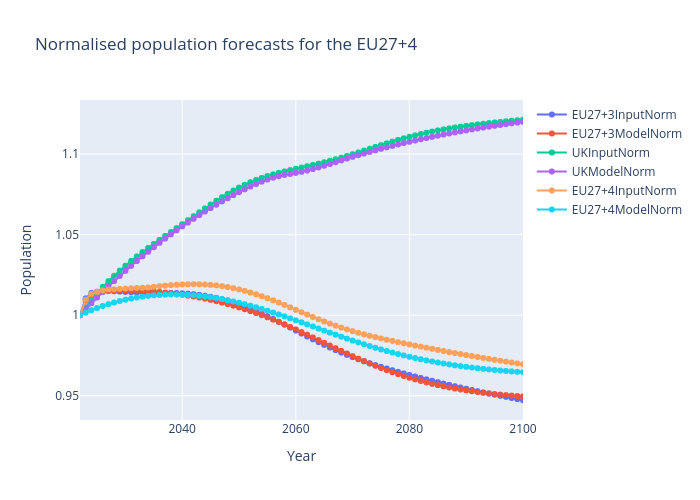
\includegraphics[width=\linewidth]{130quantification/external/population.png}
      \caption{Population projections for the EU27+3 and the UK}\label{fig:population} 
\end{figure}

\subsubsection{EU27 + 4}

\textbf{Data source:}~\cite{eurostat2023population}

\subsubsubsection{Population modelling results:}

The full results of the population modelling are presented in
\autoref{tab:population}.

\subsubsubsection{Highlights:}

\begin{itemize}
      \item The EU population is projected to rise from 446.7 million in 2022, peaking at
            453.3 million in 2026 (+1.5\%), before decreasing to 447.9 million in 2050 and
            further to 419.5 million in 2100.
      \item An increase of 5.8 years is expected in the median age of the EU population
            between 2022 and 2100.
      \item By 2100, the number of individuals aged 80 and over in the EU is projected to
            reach 64.0 million.
\end{itemize}

Populations evolve over time due to demographic factors: births, deaths, and
migration. Each of these factors influences the population's structure.
Presently, the EU is experiencing a trend of ageing in its population due to
the prevailing levels of fertility and mortality.

EUROPOP2023 offers deterministic projections based on `what-if' scenarios.
These scenarios are formed on anticipated courses for fertility, mortality, and
migration. A partial convergence is assumed among the countries in the
EUROPOP2023 projection concerning fertility, mortality, and migration patterns.
The methodology employed is primarily based on past projection exercises.
Furthermore, this study accounts for the impact of the COVID-19 pandemic and
the mass influx due to the conflict between Russia and Ukraine.

It is projected by Eurostat that all EU Member States and the three EFTA
countries will experience continued population ageing. The population in 2100
is predicted to be lower than in 2022, with a decline in the working-age
demographic. There's an observed trend of ageing within the elderly demographic
itself. Migration can both alleviate and accelerate the ageing process. It
depends on whether there's an influx or outflow of the working-age population.
For instance, the search for better job opportunities can lead to a
considerable outflow. Consequently, age dependency ratios are set to rise,
posing challenges for public expenditure on pensions, healthcare, and long-term
care.

\subsubsubsection{Method}

Eurostat provides international projections for the European Union (EU) and the
European Free Trade Association countries, which include Iceland,
Liechtenstein, Norway, and Switzerland. Unlike the UN's projections, Eurostat's
are deterministic in nature. Their most recent projection, dating from 2020,
presents a base variant along with four other variants, starting with the
baseline year 2019. In the base variant, it is forecasted that the EU-27
population will decline by nearly 7 percent or about 30 million people by 2100.
However, in the medium term, the population is expected to grow until 2025,
reaching about 449 million people, before reducing to 416 million by 2100.
Country-specific, sex, and age data are available in Eurostat`s database.

The final projection starts with the 2022 population divided by sex and age.
Mortality rates are applied to determine the number of deaths. Numbers for
non-EU and EU immigrants are computed. For the years 2022 and 2023, refugees
under TP are also included. Emigrants, including refugees under TP for the
years 2024 to 3033, are then subtracted. Based on this, the end-of-year
population and the working-age population are computed. Using these figures,
additional non-EU immigrants are calculated, and the end-of-year population is
re-assessed. This allows for the computation of live births, total deaths,
immigration, and emigration for 2022.

\subsubsubsection{Scenarios}

Eurostat also considers five alternative scenarios besides the baseline for
EUROPOP2023. These are: lower fertility, lower mortality, zero net migration,
decreased non-EU immigration, and increased non-EU immigration. For instance,
the lower fertility scenario posits a total fertility rate that's 20\% less
than the baseline for each projection year (2023 -- 2100). This implies fewer
live births yearly compared to the baseline. The lower mortality scenario
suggests a life expectancy at birth in 2100 that's two years more than the
baseline. Migration scenarios include zero net migration, 33\% less non-EU
immigration each year, and 33\% more non-EU immigration every year throughout
the projection horizon.

\subsubsection{UK}

\textbf{Data source:}~\cite{ons2023population}


\begin{itemize}
      \item New data will be released January 2024.
      \item No scenarios were developed due to the additional uncertainty in the underlying
            data related to the CoViD-19 pandemic-related fluctuations.
\end{itemize}

\subsubsubsection{Population modelling results:}

The full results of the population modelling are presented in
\autoref{tab:population}.

\subsubsubsection{Population Projections}

The UK population in mid-2020 was estimated at 67.1 million. Over the decade to
mid-2030, it's projected to rise by 2.1 million (3.2\% increase), in comparison
to a 6.9\% increase between 2010 and 2020. Over the next 25 years, the
projected growth is 3.9 million (5.8\%), less than the 15.6\% growth between
mid-1995 and mid-2020.

In contrast to the EU27+3, the UK population is projected to continue to
continue growing (slowly) until 2100, the end of the projection period, when it
reaches 76 million.

\subsubsubsection{Assumptions:}
\begin{itemize}
      \item Long-term averages are based on a 22-year period, excluding the 1990s.
      \item Long-term average falls within the ranges given by expert advisory feedback.
      \item Estimated international migration data is used for the years ending mid-2021
            and mid-2022.
      \item Linear interpolation is used from mid-2022 up to mid-2026.
      \item A three-year average of data from mid-2020 to mid-2022 is used for starting the
            linear interpolation for mid-2022.
      \item UK completed family size to reach 1.59 children per woman by 2045.
      \item Annual improvement in UK mortality rates will be 1.2\% for most ages by 2045.
      \item Net international migration to the UK will average +205,000 from mid-2027
            onwards.
\end{itemize}

\subsubsubsection{Methodology}
Projections are produced for successive years from one mid-year to the next. Age-based calculations are made to account for net migration, deaths, and births. Details such as migration timing, death rates, birth rates, and the ratio of male-to-female births are factored into the calculations. Projections are made for each UK country and then aggregated for broader regions.

\subsubsubsection{Strengths and Limitations}
Projections are based on the latest available data but are not forecasts. The inherent uncertainty in the data and the unpredictability of future events means projections may not align with future outcomes. Factors like political and economic changes can also impact population growth, and events like the UK leaving the EU or the COVID-19 pandemic are not explicitly factored in. While this bulletin focuses on projections up to mid-2045, the data includes projections up to mid-2120, which have greater inherent uncertainty.

\subsubsubsection{Merging the EU27+3 and the UK into a unified population model}

As the world undergoes the demographic transition, the relevance of Verhulst's
logistic model has resurged, providing an adequate representation of current
population growth trends. This logistic population growth dynamic is critical
for achieving global sustainable development.

These projections are informed by the finite reserves of primary exhaustible
resources and the ongoing trend of declining birth rates. These indications
suggest a shift towards a new equilibrium state for the planet that aligns with
heightened industrial and technological capacities and improved healthcare
standards. By constructing logistic models that depict the growth dynamics of
the global population and individual continents, we can forecast population
sizes and their growth rates for the next two centuries. The insights garnered
present opportunities for the regulation and optimal management of global
demographic resources.

\subsubsection{Projection Methodology}

\textbf{Methodology source:}~\cite{vanella2020populationprojections}

Population projections underpin many political and economic decisions at
various levels. Often, the users lack the expertise to fully grasp the methods
and limitations of the projections they rely on.

Population development is contingent upon three primary factors: fertility, net
migration, and mortality. Usually, a projection starts with the age- and
sex-specific numbers at a given time. Using estimates for the future
development of the three determinants, the population is projected forward.
Forecasts often refine mortality and migration by age and sex.

Projection methodologies fall into deterministic and stochastic categories.
Deterministic models, being the most widespread, set parameters in one or more
scenarios. Their strengths lie in ease of use, adaptability to changes in
parameters, and straightforwardness for non-experts. A prominent deterministic
method is the cohort component method (CCM) which separately simulates
fertility, migration, and mortality before integrating them into a projection.
Given a population \(P_{t-1}\) at the end of period \(t-1\), the CCM updates
this using births \(B_t\), net migration \(M_t\), and deaths \(D_t\) as:

\[ P_t = P_{t-1} + B_t + M_t - D_t \]

However, deterministic models face challenges. They:
\begin{itemize}
      \item Overlook the probabilistic nature of population processes.
      \item Rely on rigid future assumptions with low individual probabilities of
            occurrence.
      \item Limit the number of considered scenarios, inadequately reflecting future risk.
      \item Lack probabilistic quantification for identified futures.
      \item May be biased by experts' subjective assessments.
\end{itemize}

In contrast, stochastic models view parameters as random variables. While
deterministic models might assume fixed values for determinants like \(G_t,
M_t\), and \(S_t\) in certain scenarios, stochastic models see these as
probabilistic, represented as:

\[ \tilde{B}_t = \tilde{B}_{t-1} + \tilde{G}_t + \tilde{M}_t - \tilde{S}_t \]

Yet, it's essential to understand that no forecast offers absolute truth. Their
aim isn't predicting unexpected events, but extrapolating core demographic
trends. Both deterministic and stochastic methods exist to quantify forecast
uncertainty.

Applying these results in real-world scenarios warrants a cautious approach.
Past trends might not persist in the future. For instance, population growth
isn't just about demographics but also infrastructure. Can a housing market
accommodate growth? Will cities meet their limits? Projections inherently carry
assumptions. For instance, regions must meet housing demands, and urban
challenges arise from positive population growth, such as the need for expanded
childcare or public transport infrastructure.

Predicting and managing future global population growth stands as a paramount
challenge for humanity. Most contemporary researchers believe there's a ceiling
to the planet's `carrying capacity'. Come 2022, Earth's population is
anticipated to hit the eight billion mark. UN predictions suggest that by 2100,
this number will rise to ten billion. However, there's an observable trend
towards smaller family sizes, with birth rates currently hovering around the
replacement rate of 2.1 children per woman. Should global fertility rates align
with family replacement levels (2.0) by 2100, Earth's population is projected
to stabilise between ten and eleven billion. The emergence of new statistical
data necessitates updates to global population growth models. Where once the
Verhulst logistic model was deemed inadequate for characterising global
population growth dynamics, the tapering growth rate now reaffirms its
applicability. Many recent studies have leveraged the logistic growth model.
Our analyses confirm that Earth's population growth rate aligns closely with a
quadratic function, mirroring the Verhulst equation (Fig. 4). All subsequent
computations will employ the Verhulst logistic model:

\begin{equation}
      \frac{dY}{dt} = a \cdot Y - b \cdot Y^2
\end{equation}

The solution to equation (8) will be sought as a logistic function:

\begin{equation}
      Y = g + \frac{b}{1 + A \exp(-a(t - t_0))}
\end{equation}

Function \( Y(t) \) parameters were ascertained using the least squares method,
ensuring maximal alignment between the function's value and the existing
statistical data. The parameter \( g \) was presumed equal to the initial
population size at the start of observations (\( t_0 =1900 \)).

\subsubsubsection{Curve Fitting Explanation}

Terms with subscript 1 describe the initial logistic component, charting
population growth from 2022 to 2042.

Subscript 2 terms Correspond to the second logistic component, which outlines
post-2042 population decline.

\begin{description}[style=nextline, leftmargin=2cm]
      \item[\(\mathbf{b_1}\)] 
            Represents the initial population at the start of the observation period - Europe's population in 1900 per the model's parameters.

      \item[\(\mathbf{b_1}\)] 
            Denotes the carrying capacity of population growth, effectively indicating the population apex achievable via the first logistic function.

      \item[\(\mathbf{A_1}\)] 
            Influences the gradient of the first growth phase. Higher values result in steeper population inclines.

      \item[\(\mathbf{a_1}\)] 
            Represents the growth rate of the initial logistic function, dictating how swiftly the population nears the carrying capacity \( b_1 \).

      \item[\(\mathbf{t_1}\)] 
            Marks the inflection point in the first logistic phase, signifying the period of maximum growth velocity.

      \item[\(\mathbf{b_2}\)] 
            Illustrates the decline's carrying capacity, indicating the population decrease as projected by the second logistic function.

      \item[\(\mathbf{A_2}\)] 
            Determines the gradient of the decline phase, with larger values resulting in sharper declines.

      \item[\(\mathbf{a_2}\)] 
            Represents the rate of decline in the latter logistic function, determining the speed at which the population reaches the decline's carrying capacity \( b_2 \).

      \item[\(\mathbf{t_2}\)] 
            Highlights the inflection point during the decline phase, marking the period where the decrease is most rapid.
\end{description}


\begin{table}[h!]
      \centering
      \small
      \caption{Population projections for the EU27+4}\label{tab:population}
      \begin{tabular}{|C{1.5cm}|C{1.5cm}|C{1.5cm}|C{1.5cm}|C{1.5cm}|}
            \hline
            \rowcolor{headerblue} % Applying the header color
            \textcolor{white}{\textbf{YEAR}} & \textcolor{white}{\textbf{MEDIAN AGE}} & \textcolor{white}{\textbf{EU27+4} (million)} & \textcolor{white}{\textbf{EU27+3} (million)} & \textcolor{white}{\textbf{UK} (million)} \\
            \hline
            \csvreader{csvs/population.csv}{}{\csvcoli& \csvcolii& \csvcoliii& \csvcoliv& \csvcolv\\ \hline}
      \end{tabular}

\end{table}



\clearpage
\subsubsection{Incorporation of demographic factors into individual waste stream models}


\boxws{This section will be filled out with the details of exactly how the demographic parameters are incorporated into your stock and flow models}


\wasteSubsubsubsecBATT
\begin{itemize}
    \item X
\end{itemize}

\wasteSubsubsubsecCDW
\begin{itemize}
    \item X
\end{itemize}

\wasteSubsubsubsecELV
\begin{itemize}
    \item X
\end{itemize}

\wasteSubsubsubsecMIN
\begin{itemize}
    \item X
\end{itemize}

\wasteSubsubsubsecSLASH
\begin{itemize}
    \item X
\end{itemize}

\wasteSubsubsubsecWEEE
\begin{itemize}
    \item X
\end{itemize}


\subsubsection{Conclusion}


\boxreview{This conclusion will be compiled once the individual waste stream sections for each parameter are complete.}


\sectionEndlines
\clearpage

\clearpage
\subsection{Economic factors: \textit{GDP growth}}\label{sec:quantification_economic}

\subsubsection{Definitions}

\begin{description}[style=nextline]
  \item[Gross Domestic Product (GDP) PPP]
        A measure of a country's economic output that accounts for differences in price levels between countries. By using PPPs and the common currency of international dollars, GDP PPP is adjusted for price level differences across countries, providing a more accurate measure of the economic output and living standards, as it reflects the real purchasing power of the citizens.

  \item[Purchasing Power Parity (PPP)]
        An economic theory that allows the comparison of the purchasing power of various world currencies to one another. It involves a comparison of the relative prices of a standard set of goods and services in different countries, thus providing a measure of the relative cost of living and enabling a more accurate comparison of economic well-being.
\end{description}

\boxparameter{GDP growth}{Slow stable growth}{Slow stable growth}{Slow stable growth}



\subsubsection{Sources of data}

The GPD projections for FutuRaM's future scenarios are based on economic data from the OECD as well as population data from Eurostat and the UK's ONS~\cite{oecd2021gdpdata,eurostat2023population,ons2023population}

\subsubsection{Results of projections}

As an `external element', the GDP projections do not differ across the scenarios, only as a function of time.

The results of the projections are shown in~\autoref{fig:gdp-projections}. An interactive figure can be viewed \href{https://futuram-project.github.io/FutuRaM.github.io/WP2/assets.html}{here~\faLink}

\begin{landscape}
\begin{figure}[h!]
    \centering
    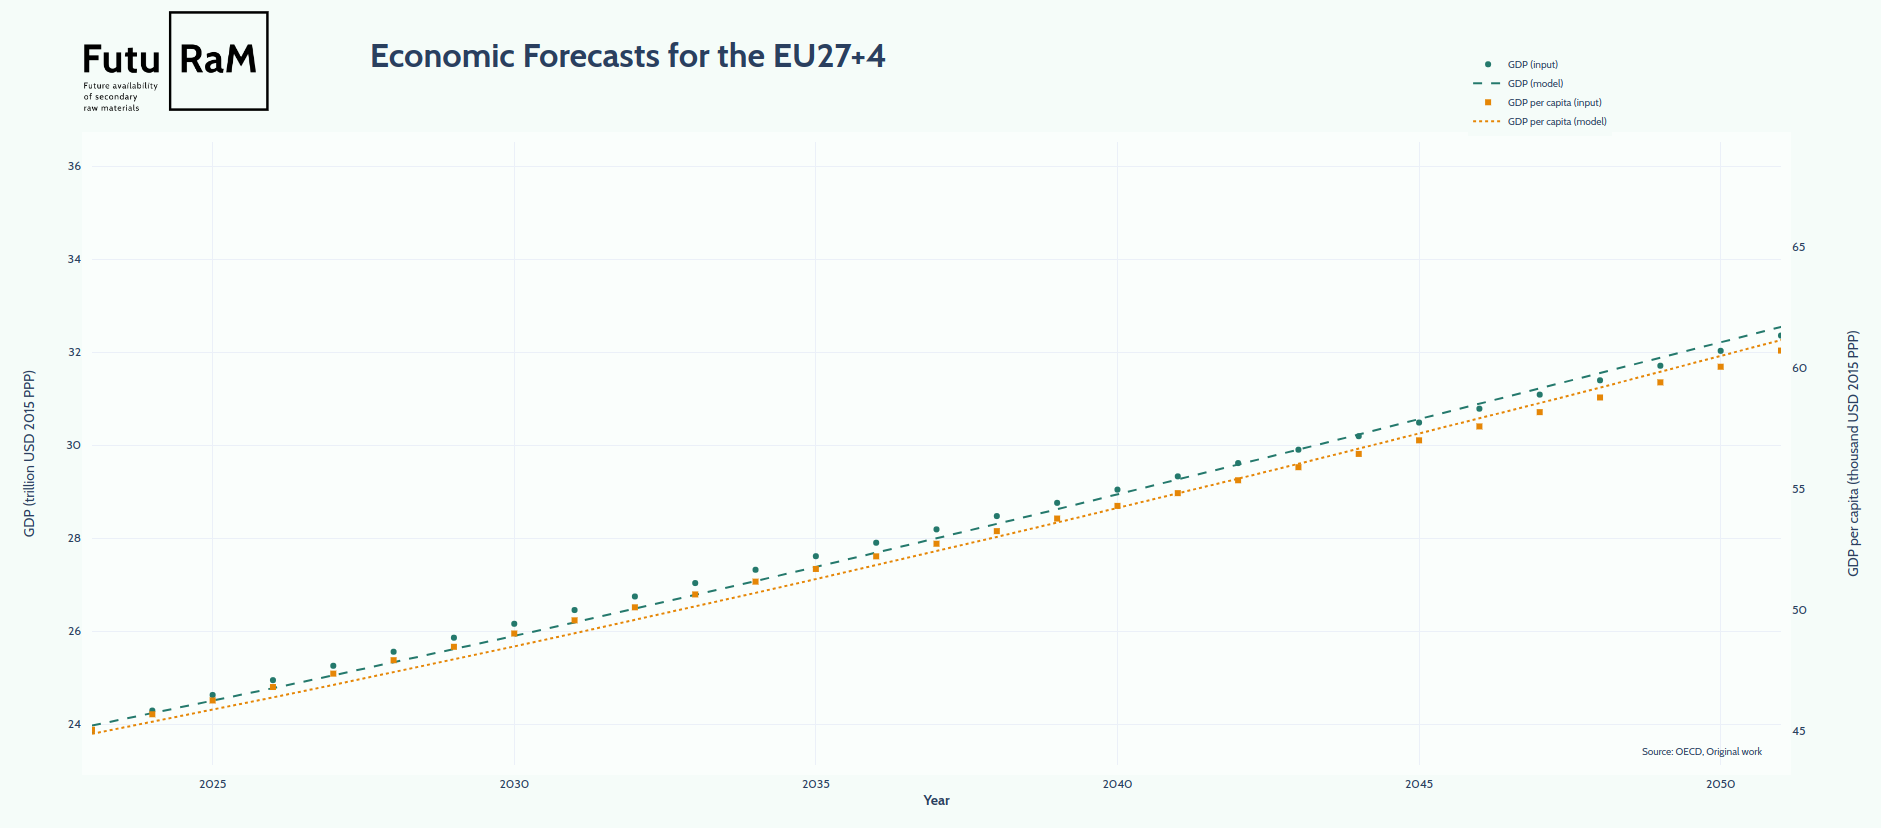
\includegraphics[width=\linewidth]{130quantification/external/gdp.png}
    \caption{GDP projections for the EU27+4}\label{fig:gdp-projections}
\end{figure}
\end{landscape}
\FloatBarrier

\subsubsection{Methodological Overview of OECD's GDP Projection Framework}~\cite{oecd2021gdpdata, oecd2021gdpmethod,duval2010gdp, oecd2012gdp}

The OECD's approach to projecting GDP is rooted in the principle that income levels across various nations will gravitate towards those observed in the most advanced economies, an idea put forth by~\cite{barro2004gdp, barro2004gdpbook}. This convergence is modelled through an enriched version of the Solow growth model, factoring in a dual-sector configuration~\cite{mankiw1992gdp}, which the OECD dubs the ENV-Growth model. Rather than focusing solely on convergence in income, the ENV-Growth model prioritises the growth factors that will drive GDP over time.

For GDP projections up to 2060, the OECD combines model-based assessments with expert evaluations, considering the economic dynamics of individual countries and the global market. These forecasts are denominated in the constant US dollars and PPPs of 2010, based on data from OECD and World Bank, which use the Atlas method for calculating PPPs~\cite{worldbank2023gdp,oecd2021gdpmethod}. The data originate from the OECD Long-Term Baseline Scenario. This scenario, which is integral to the OECD Economic Outlook, serves as a comparative standard to gauge the possible effects of structural reforms, assuming a policy-neutral environment. Conversely, long-term projections diverge from the medium-term forecasting model, which is predominantly demand-driven, by focusing on a supply-side perspective that takes into account labour and capital availability and productivity growth rates.



\subsubsection{Determinants of Long-term Growth}~\cite{fontagne2022gdp, oecd2021gdpmethod}


Recognizing the multifaceted nature of economic advancement, GDP growth projections consider an array of influences such as demographics, educational attainment, technological progress, energy access, and capital flow patterns. The MaGE framework facilitates GDP estimation by charting dynamic paths that reflect the structural interplay defining the economic landscape until 2050~\cite{fontagne2022gdp}.

The ENV-Growth model's projections span a century and include a wider selection of countries, enhancing the original methodologies developed by the OECD Economics Department~\cite{duval2010gdp, oecd2012gdp}. It introduces considerations for energy usage and resource revenue from oil and gas sectors, aligning with the enhanced sectoral approach for fossil fuels presented by~\cite{chateau2012gdp}.


The model's foundation lies in its projection of the five pivotal elements driving economic growth:

\begin{itemize}
  \item Physical capital
  \item Employment, shaped by population trends, age demographics, participation rates, and unemployment scenarios
  \item Human capital, based on education and its consequential effect on labour productivity
  \item Energy demand and resource extraction for exporting countries
  \item Total factor productivity (TFP)
\end{itemize}

The determinants of growth are not restricted to these factors; they also encompass a spectrum of social, economic, and institutional influences, including workforce education, trade openness, institutional integrity, fiscal strategies, regulatory frameworks, and demographic shifts. The underlying potential for economic catch-up through technology transfer and innovation is underscored by the differential in income between each country and the global technology frontrunner.

In the context of employment, projections from IIASA inform the total employment figures, combining time-specific participation rates for different age cohorts with projected unemployment trends. Education assumptions translate gender and age-specific educational projections into a human capital index, which then informs labour productivity enhancements.

For physical capital, the model follows a standard capital accumulation methodology with a set depreciation rate, with the investment rate per unit of GDP edging towards a balanced growth path level determined by the production function's structural parameters.

Energy and natural resources are integrated as productive components for consumers and as extra income from specific oil and gas sectors for producer nations. The model calibrates domestic energy productivity to historical improvement rates, progressing towards an efficiency frontier indicative of cutting-edge energy appliances. The economic contribution of energy resources to producer countries is extrapolated from resource depletion models that describe the dynamics between reserves and resources and the temporal evolution of marginal production costs.

FutuRaM's economic forecasts, while not based directly on the SSP data, are consistent with the SSP2 baseline derived from similar sources and models~\cite{ssp2017narrative, jiang2017ssp, leimbach2017ssp, cuaresma2017ssp, dellink2017ssp, samir2017ssp}, offering a comprehensive picture of potential economic trajectories.


\begin{figure}[h!]
  \centering
  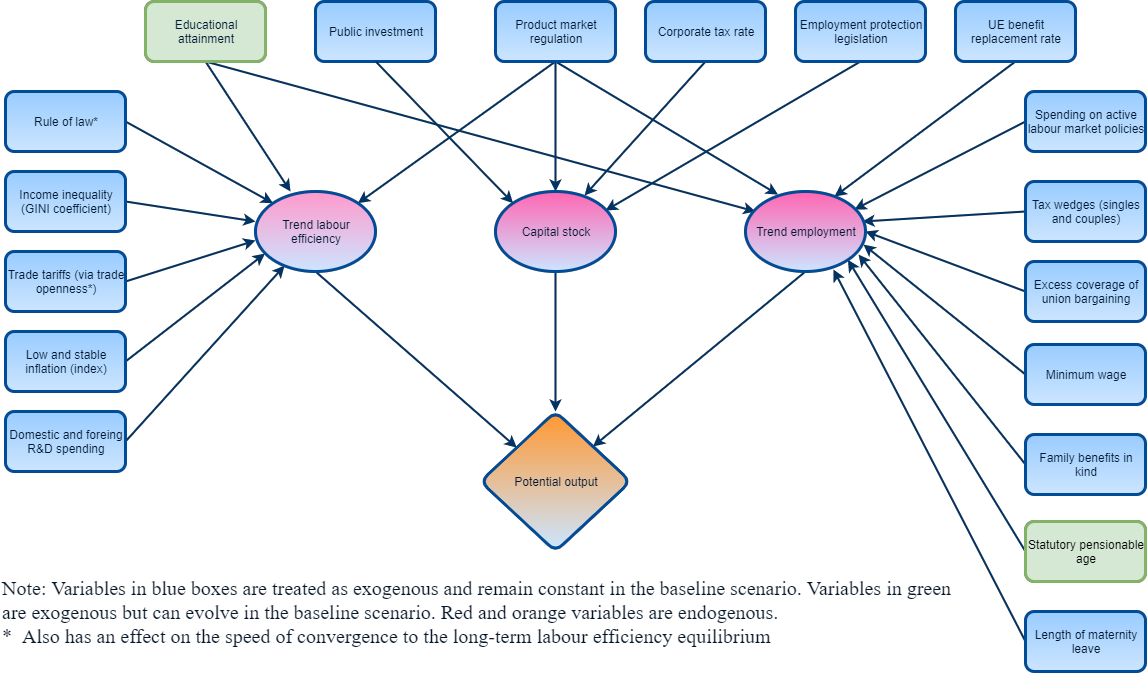
\includegraphics[width=\textwidth]{130quantification/external/oecd2021gdpmethod_drivers.png}
  \caption[Factors incorporated in the long-term GDP model]{Factors incorporated in the long-term GDP model~\cite{oecd2021gdpmethod}}\label{fig:gpd_method}
\end{figure}

\clearpage
\subsubsection{Implications of GDP Growth on FutuRaM's Waste Models}

GDP growth has significant implications for models concerning secondary raw material recovery and waste generation. For example, increasing GDP tends to lead to higher consumption levels, which can result in more waste generation across various streams. However, higher income also provides greater resources for investment in recovery technologies and infrastructure. Below are some examples for each of the specified waste streams.

\wasteSubsubsubsecBATT

As GDP grows, the demand for electronic devices and electric vehicles typically increases, leading to a higher turnover of batteries. This could necessitate advancements in recovery methods for battery components, such as lithium and cobalt, to reduce reliance on primary sources and mitigate environmental impact.

\wasteSubsubsubsecCDW

Economic growth often spurs construction activity, thereby increasing CDW. Increasing GDP as a ratio of waste generation could lead to enhanced recycling processes, promoting the circular economy by converting waste into secondary raw materials for new construction projects.

\wasteSubsubsubsecELV

The number of ELVs rises with economic prosperity, as people can afford newer vehicles more often. This creates opportunities to recover valuable materials and components, necessitating more efficient recycling processes.

\wasteSubsubsubsecMIN

As economies expand, so does the demand for minerals, potentially increasing mining waste. With increased GDP, there could be more investment in techniques to minimise waste generation and recover valuable materials from mining by-products.

\wasteSubsubsubsecSLASH

Higher GDP can correlate with increased industrial activity, producing more slags and ashes. Enhanced recovery techniques can transform these by-products into useful secondary raw materials, such as aggregates in construction.

\wasteSubsubsubsecWEEE

GDP growth can lead to shorter replacement cycles for electronic goods, increasing the amount of WEEE. There's a potential for improved recovery of precious metals and rare earth elements, driving innovation in e-waste recycling technologies.

\clearpage

\subsubsection{Incorporation of economic growth into individual waste stream models}

\boxws{This section will be filled out with the details of exactly how this parameter is incorporated into your stock and flow models}

\wasteSubsubsubsecBATT
\begin{itemize}
    \item X
\end{itemize}

\wasteSubsubsubsecCDW
\begin{itemize}
    \item X
\end{itemize}

\wasteSubsubsubsecELV
\begin{itemize}
    \item X
\end{itemize}

\wasteSubsubsubsecMIN
\begin{itemize}
    \item X
\end{itemize}

\wasteSubsubsubsecSLASH
\begin{itemize}
    \item X
\end{itemize}

\wasteSubsubsubsecWEEE
\begin{itemize}
    \item X
\end{itemize}



\subsubsection{Conclusion}

Economic growth can therefore act as both a driver of waste generation and a catalyst for innovation in the recovery of secondary raw materials. The challenge for models like FutuRaM lies in accurately predicting these trends and proposing effective strategies to balance economic benefits with environmental sustainability.

\boxreview{This conclusion will be more completely compiled once the individual waste stream sections for each parameter are complete.}

\sectionEndlines

\clearpage


\clearpage
\subsection{The Renewable Energy Transition}\label{sec:external-energy_transition}


\subsubsection{Definition}

The term "energy transition" refers to the current global shift from fossil fuels to renewable energy sources to meet the urgent need to reduce greenhouse gas emissions, combat climate change, and enhance energy security. This transition encompasses a fundamental transformation of energy supply and consumption patterns, including the increased use of sustainable energy to achieve a low-carbon economy. Historical shifts in energy sources—from biomass to coal, and later to oil and natural gas—reflect the ongoing evolution of energy use. The present focus is on scaling up renewables such as solar and wind, which are becoming increasingly cost-competitive. Key aspects of the transition include adopting electric vehicles, improving public transportation, advancing energy-efficient technologies for building heating, and developing energy storage and grid solutions to support the integration of variable renewable energy sources.

\subsubsection{Future energy mix in the EU}

The projected electricity mix for the EU is presented in \autoref{fig:energy_mix}. An interactive figure can be viewed \href{https://futuram-project.github.io/FutuRaM.github.io/WP2/assets.html}{here~\faLink}

\begin{figure}[h!]
    \centering
    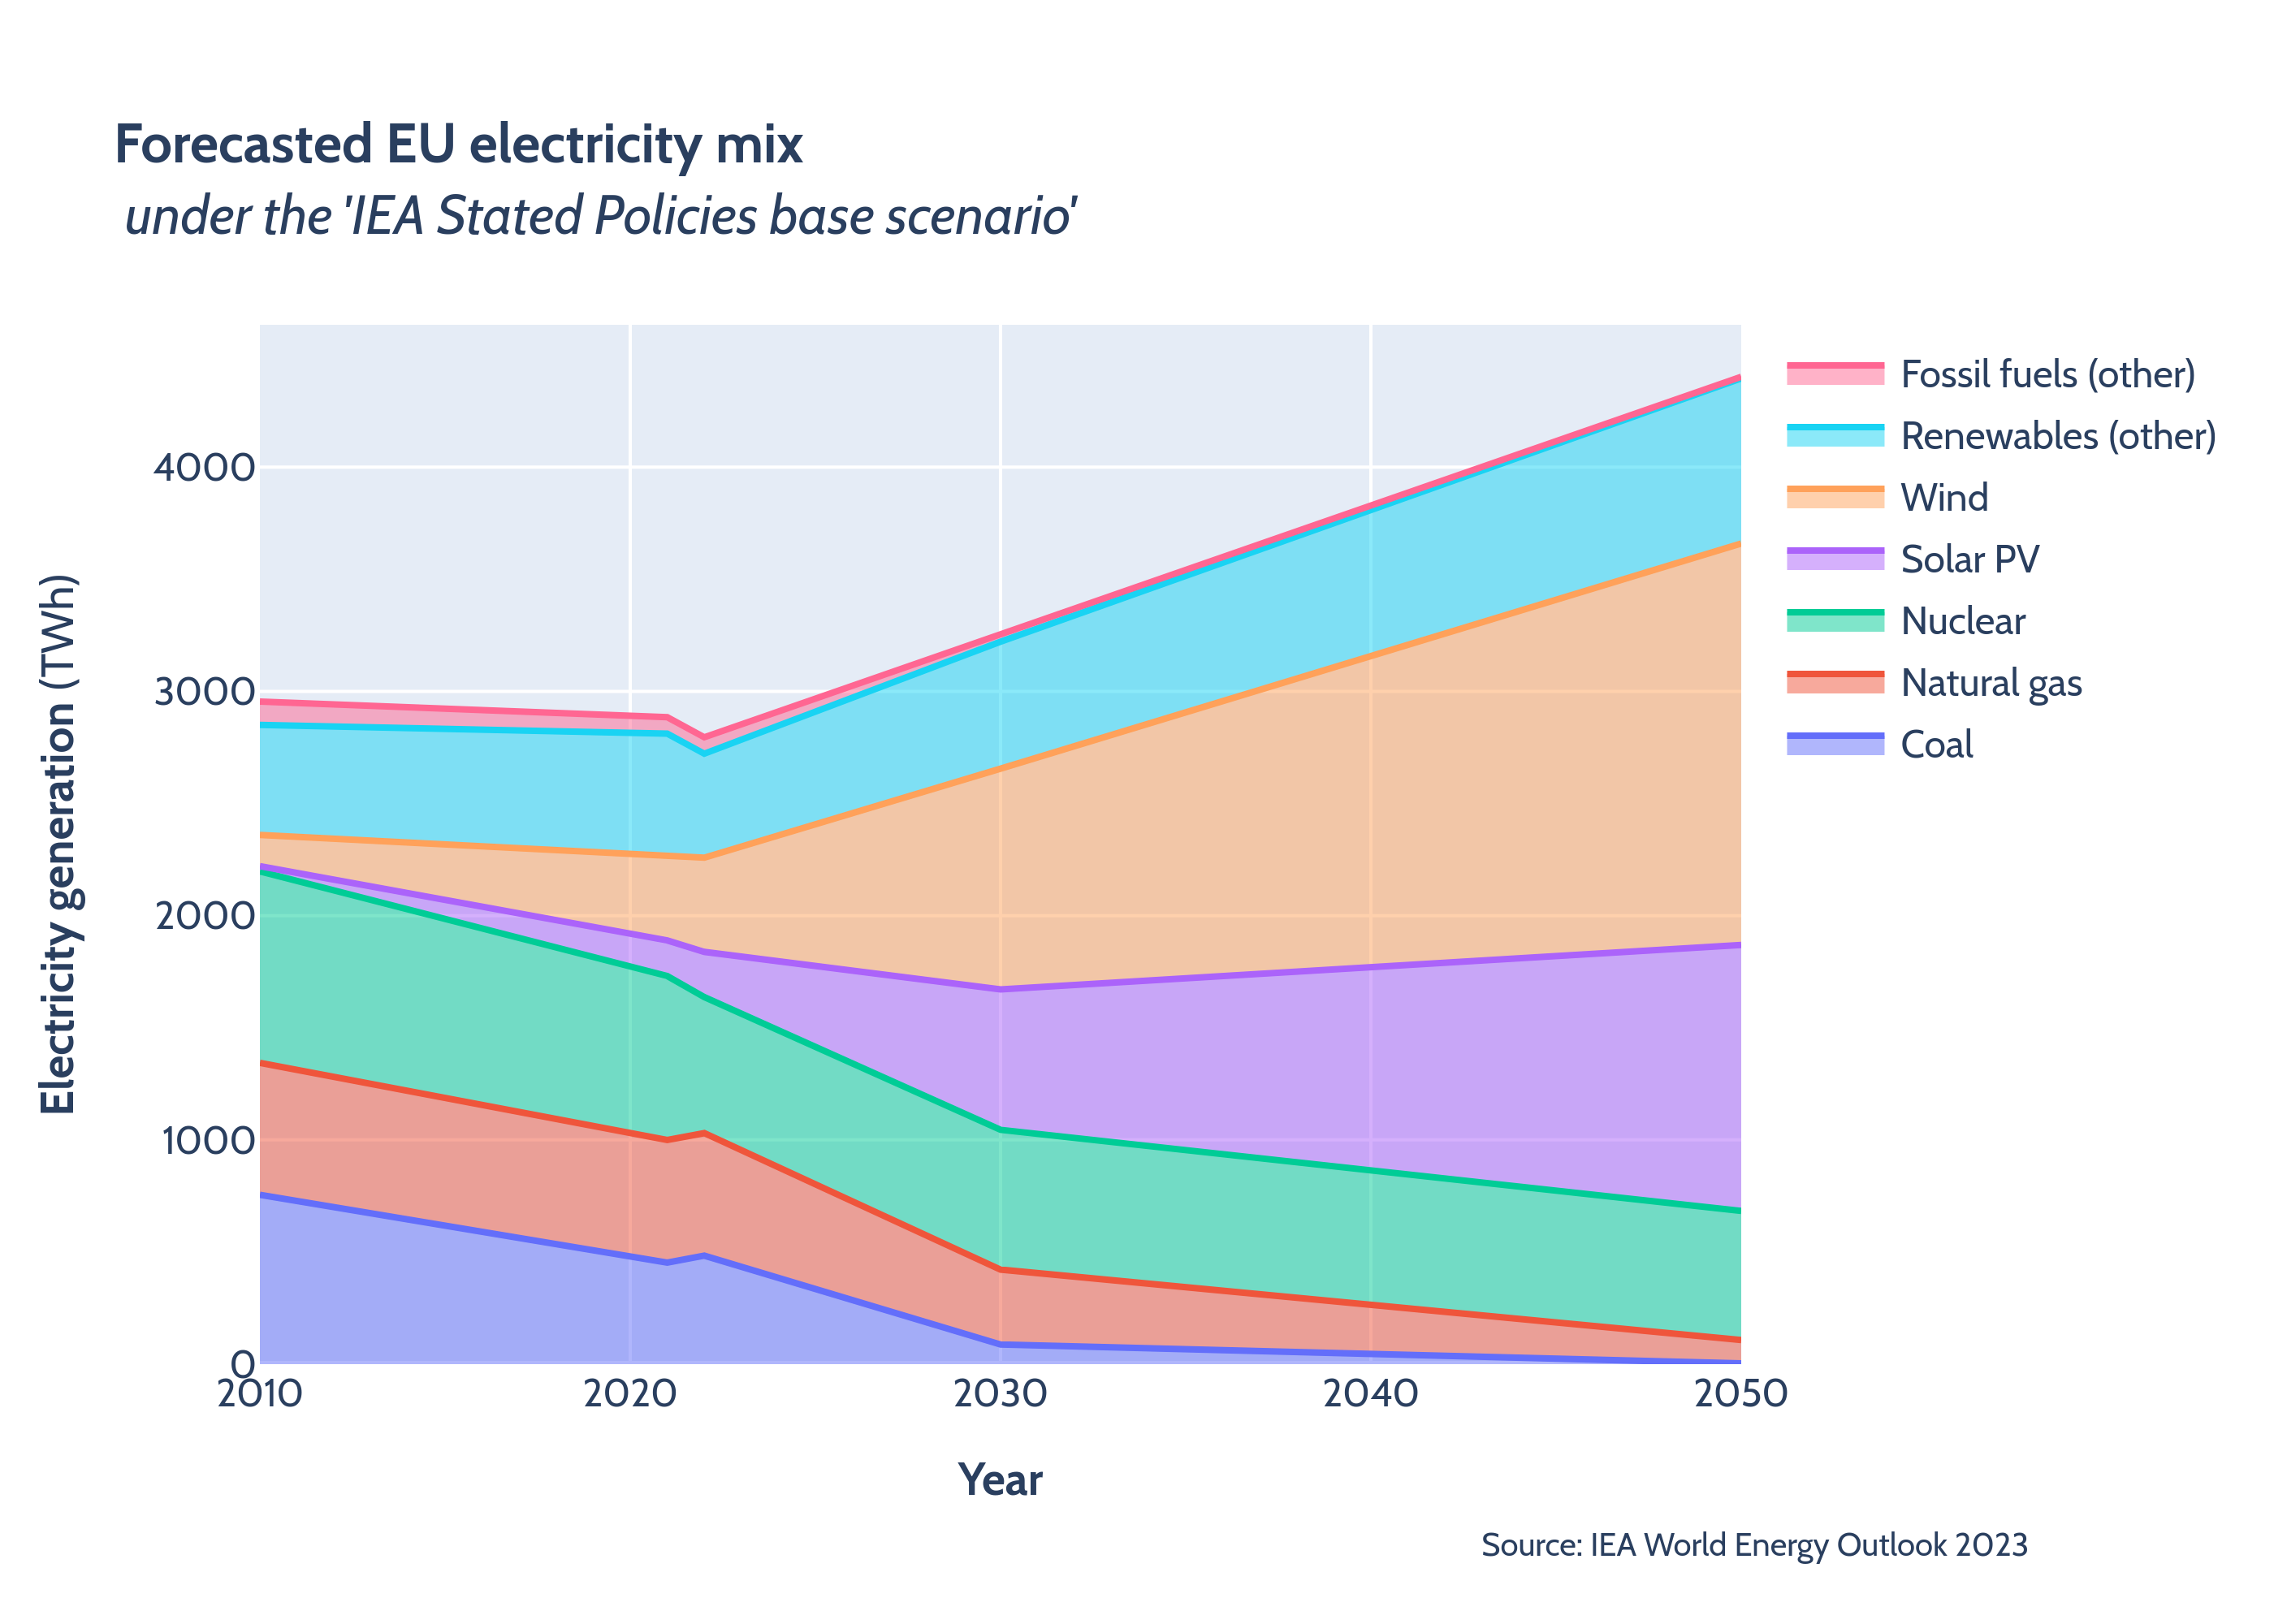
\includegraphics[width=\textwidth]{130quantification/external/energy_mix_forecast.png}
    \caption{EU electricity mix forecast until 2050}\label{fig:energy_mix}
\end{figure}

\subsubsection{Brief context of renewable energy in the EU}

Renewable energy is integral to the EU's shift towards a low-carbon economy and reducing reliance on imported fossil fuels—a response accentuated by the urgency to curtail dependence on Russian energy sources. The EU's strategic move is encapsulated in the REPowerEU Plan of Action, introduced in May 2022, and agreed upon in 2023 which prescribes an aggressive uptake of renewables, emphasizing wind and solar PV, alongside hydrogen, heat pumps, and batteries, vital for energy storage and transportation decarbonisation \cite{jrc2023supplychain,eu2023energy,eu2022repower, jrc2022energyclimateoutlook}.

In analysing the renewable sector in FutuRaM, the focus is on solar PV, wind turbines, electrolysers, batteries, and residential heat pumps. Other renewable sources like bioenergy, hydro, geothermal, and ocean energy, while part of the portfolio, are expected to have minimal impact on critical materials demand and are not central to this analysis.

\subsubsection{Justification for setting as an external scenario factor}

The ongoing global energy transition is a profound shift that holds implications for almost every facet of society, especially regarding CRMs, other raw materials and the system of waste management. This transition from fossil fuels towards renewable energy sources demands a significant increase in various CRMs, influencing their supply and demand curves extensively. In the development of FutuRaM's scenarios, the energy transition is recognised as a fundamental driver of change. However, for the purposes of focussed and strategic scenario modelling, it has been categorised as an external factor.

This classification allows for a delineation between direct policy levers within the purview of SRM systems and broader macro-environmental trends that, while influential, are not the primary subject of analysis within FutuRaM. As such, the project's scenarios incorporate a consistent baseline projection of the energy transition's effects, shared across the three scenarios, ensuring that the core analysis remains centred on material-centric policy outcomes and targets of the CRM act. This ensures that the resulting insights are actionable and tailored to the nuances of material management and recycling systems. It reflects a strategic choice to maintain scenario tractability and avoid the dilution of policy implications that could arise from an overly broad scope of variables.

Moreover, the scenario architecture within FutuRaM is constructed with inherent flexibility, permitting later incorporation of amendments to the background energy transition trends. This adaptability is essential to ensure that, as the energy landscape evolves and new data becomes available, the scenarios can be revised and updated, thereby preserving the relevance and accuracy of the project's findings over time.


\subsubsection{Relevant technologies in the renewable energy sector}

The cornerstone technologies in renewable energy—batteries, electrolysers, wind turbines, heat pumps, and solar PV—play pivotal roles across various sectors (Figure 85). Heat pumps serve industrial processes, while solar PV and batteries support ICT, defence, and mobility with energy and uninterrupted power supplies, respectively \cite{jrc2023supplychain}.

Wind energy, expected to surge, will benefit from cost-efficient, innovative turbines designed for increased productivity in offshore and low-wind conditions. Projections from GECO present two scenarios: a conservative estimate shows wind capacity expanding from 732 GW (2020) to 1,400 GW (2030), and to 4,050 GW by 2050. An optimistic forecast anticipates a rise to 2,500 GW by 2030 and 8,400 GW by 2050.

Solar PV is poised for exponential growth due to advancements enhancing efficiency and lowering costs. GECO's cautious scenario predicts growth from 710 GW (2020) to 2,950 GW (2030), reaching 7,500 GW by 2050. The optimistic scenario projects a tenfold increase by 2030 and sixteenfold by 2050 compared to 2020 levels.

Addressing the intermittency of wind and solar power necessitates adequate storage solutions and robust grid systems, with electrolysers emerging as a crucial technology for renewable hydrogen production, forecasted to exceed 1 GW capacity by the end of 2022 \cite{iea2022renewables}.

Additionally, digitalisation, robotics, and 3D printing are set to boost the renewable sector's productivity and optimisation across its value chain. Heat pump sales are also on an upward trend, with a peak expected in 2045, ranging between 15 million (low demand) and 38 million units (high demand) by 2050.

Material demand in the renewable sector is dominated by wind turbines, electrolysers, and solar PV, with wind energy leading in consumption of critical materials.


\subsubsection{Supply Chain bottlenecks in renewable energy}

Supply chain bottlenecks present a significant challenge in the deployment of renewable energy technologies, particularly for wind turbines, solar PV, electrolysers, and heat pumps. The production of NdFeB permanent magnets for wind turbines demands rare earth elements (REEs) like neodymium, dysprosium, praseodymium, and terbium, with the EU being highly dependent on imports for both raw and processed materials such as permanent magnet alloys and components like blades.

Solar PV technologies necessitate strategic raw materials, including silicon metal and rare metals like gallium and germanium, with China dominating the production of silicon ingots and wafers. This reliance on imports extends across the value chain, including the crystalline silicon cell production where the EU's contribution is minimal.

The battery industry utilizes strategic raw materials such as lithium, manganese, and cobalt, with raw materials and components largely imported. A shift is anticipated towards nickel-rich batteries or alternative chemistries to reduce reliance on high-cobalt-content lithium-ion batteries (LIBs) due to the oligopoly control of critical components in Asia.

Electrolysers for hydrogen production use a range of strategic raw materials, particularly from the platinum group metals (PGMs), but also silicon metal, aluminium, copper, and magnesium, with the EU facing challenges in sourcing these materials. For heat pumps, strategic raw materials needed include magnesium and copper, but no significant bottlenecks have been identified, with most critical materials used in microchips and IT controllers.

Across all technologies analysed, a common pattern of heavy reliance on imports, particularly from China, is observed at different stages of the value chains. The EU’s primary sourcing and processing capabilities for critical raw materials are notably low, creating dependencies at multiple levels. Despite a strong manufacturing capacity for wind turbine assembly, the EU is entirely reliant on imports for the value chain of rare-earth permanent magnets. Similarly, for solar PV, the dependence on imports is comprehensive. The recent surge in Chinese manufacturing market share for heat pumps and the developing value chain for batteries in the EU are also noteworthy.

A breakdown of the materials required for each technology is given in \autoref{tab:energy-crms}.


\newgeometry{left=2cm,right=2cm,top=2cm,bottom=2cm}
\begin{landscape}
    \centering
    \small
    \renewcommand{\arraystretch}{0.8} % adjust the value as needed
    \begin{longtable}{|C{2cm}|L{3cm}|C{2cm}|C{2cm}|C{2cm}|C{2cm}|C{2cm}|C{2cm}|}
        \caption{Raw materials essential to the renewable energy sector}\label{tab:energy-crms}\\
        \hline
        \rowcolor{headerblue} % Applying the header color
        \color{white}\textbf{SUPPLY RISK} & \color{white}\textbf{MATERIAL} & \color{white}\textbf{CRM} & \color{white}\textbf{BATT} & \color{white}\textbf{H2} & \color{white}\textbf{WIND} & \color{white}\textbf{SOLAR (PV)} & \color{white}\textbf{HEAT PUMPS} \\
        \hline
        \endfirsthead%
        \hline
        \multicolumn{8}{r}{\textcolor{headerblue}{\textit{{Continued on next page}}}}\\
        \endfoot%
        \rowcolor{white}
        \multicolumn{8}{c}{{\textcolor{headerblue}{\textit{\tablename\ \thetable{} --- Continued from previous page}}}}\\
        \hline
        \rowcolor{headerblue} % Applying the header color
        \color{white}\textbf{SUPPLY RISK} & \color{white}\textbf{MATERIAL} & \color{white}\textbf{CRM} & \color{white}\textbf{BATT} & \color{white}\textbf{H2} & \color{white}\textbf{WIND} & \color{white}\textbf{SOLAR (PV)} & \color{white}\textbf{HEAT PUMPS} \\
        \endhead%
        \bottomrule
        \endlastfoot%
        \csvreader[separator=comma, late after line=\\]{csvs/energy-crms.csv}{}{
            \csvcoli & \csvcolii & \csvcoliii & \csvcoliv & \csvcolv & \csvcolvi & \csvcolvii & \csvcolviii
        }
    \end{longtable}
    \renewcommand{\arraystretch}{1} % reset \arraystretch to its original value
    \end{landscape}
\restoregeometry% restore margins to normal


The integration of the energy transition has significant implications for the management of Critical Raw Materials (CRMs) across various waste streams due to changing material requirements and waste profiles~\cite{jrc2023supplychain,jrc2020reedemanddata,iea2023energytechperspectives,iea2023crm}.

\vspace{\baselineskip}
\textbf{For example:}

\wasteSubsubsubsecBATT
\vspace{-1cm}
\begin{itemize}
    \item Increased deployment of Li-ion batteries for energy storage will lead to a surge in waste batteries, necessitating improved recycling technologies to recover CRMs.
    \item The transition to renewable energy sources may lead to changes in the battery composition, affecting recycling processes and the types of CRMs that need to be managed.
\end{itemize}

\wasteSubsubsubsecELV
\vspace{-1cm}
\begin{itemize}
    \item The shift towards electric vehicles will transform the composition of ELVs, increasing the relevance of CRMs used in electric powertrains and batteries.
    \item This transition requires the adaptation of ELV recycling infrastructure to efficiently process and recover new types of CRMs.
\end{itemize}

\wasteSubsubsubsecWEEE
\vspace{-1cm}
\begin{itemize}
    \item As energy systems become more digitized and interconnected, WEEE will contain a broader array of CRMs, prompting the need for more sophisticated recycling methods.
    \item The growing volume of WEEE will challenge current recycling capacity and technology, calling for significant innovation in CRM recovery techniques.
\end{itemize}

\wasteSubsubsubsecCDW
\vspace{-1cm}
\begin{itemize}
    \item Green building materials and energy-efficient technologies may introduce new CRMs into CDW, changing the material recovery landscape.
    \item The promotion of deconstruction over demolition could preserve the integrity of materials containing CRMs, allowing for better recovery rates.
\end{itemize}

\wasteSubsubsubsecMIN
\vspace{-1cm}
\begin{itemize}
    \item The drive for clean energy technologies is expected to increase the mining of specific CRMs, potentially leading to higher volumes of mining waste that must be managed sustainably.
\end{itemize}

\wasteSubsubsubsecSLASH
\vspace{-1cm}
\begin{itemize}
    \item The energy transition could increase the generation of certain industrial wastes such as slags, which may contain valuable CRMs.
\end{itemize}

\vspace{\baselineskip}
\subsubsection{Implementation in EU Law}

\subsubsubsection{Fit for 55 Package (2021)}

The "Fit for 55" package is a collection of policy initiatives proposed by the European Commission in July 2021 aimed at revising and updating EU legislation to reflect the increased ambition of reducing net greenhouse gas emissions by at least 55\% by 2030, compared to 1990 levels~\cite{eu2021fitfor55}. This target was a significant step up from the previous goal of a 40\% reduction and is part of the European Union's plan to become climate-neutral by 2050 --- an objective set out in the European Green Deal\cite{eu2019greendeal}.

The package includes proposals to revise the EU Emissions Trading System (ETS), to increase the use of renewable energy, to improve energy efficiency, and to implement carbon pricing mechanisms, among other measures. The intention is to align existing laws with the 2030 climate target and to set the legal foundation for Europe's transition to a green economy. This includes changes across various sectors including transportation, building, and energy production to reduce emissions and promote sustainable practices.

\subsubsubsection{REPowerEU Plan (2022)}

The invasion of Ukraine by Russia has caused significant disruption to energy markets in Europe and globally. To eliminate reliance on an unreliable supplier, the European Commission has devised the REPowerEU plan~\cite{eu2022repower}. This initiative focuses on energy conservation, the production of clean energy, and the diversification of energy sources, supported by financial and legal measures to develop Europe's necessary new energy infrastructure and systems.

\paragraph{Accelerating Clean Energy} Renewable energy sources, being both cost-effective and environmentally friendly, can be produced locally, thereby reducing dependency on imported energy. The REPowerEU plan aims to expedite the green transition and trigger substantial investments in renewable energy. It also seeks to facilitate the rapid transition of industry and transport from fossil fuels, reducing both emissions and dependency.

This includes a variety of measures focused on renewable energy and energy efficiency, such as:

\begin{itemize}
    \item Increasing the EU's 2030 renewable energy target of the `Fit for 55 package' from 40\% to 45\%.
    \item Accelerating the deployment of photovoltaic (PV) energy.
    \item Introducing the European Solar Rooftop Initiative.
    \item Doubling the deployment rate of individual heat pumps.
    \item Decarbonising the industry by promoting electrification and renewable hydrogen.
    \item Speeding up renewable energy project and grid infrastructure permit processes.
    \item Increasing the EU’s binding energy savings target for 2030 to 13\%.
\end{itemize}

The May 2022 REPowerEU plan by the European Commission, in response to the energy market disruptions due to Russia's invasion of Ukraine, is designed to rapidly cut down on the EU's reliance on Russian fossil fuels. It raises the renewable energy target of the Fit for 55 package from 40\% to 45\%.

This ambitious goal for renewable energy use, coupled with REPowerEU’s strategies to reduce energy demand, necessitates substantial increases in renewable capacity across the electricity, transport, and heating and cooling sectors. The Commission forecasts that to meet the 2030 objectives, renewable electricity should reach 69\%, 32\% in transport, and a yearly growth of at least 2.3 percentage points in heating and cooling.


\subsubsubsection{Renewables Energy Directive (2023)}

The recent legislation strengthening the EU Renewable Energy Directive marks an advancement towards the European Green Deal and REPowerEU ambitions. With the provisional agreement, the EU's binding renewable energy target for 2030 is now at least 42.5\%, aiming potentially to reach 45\%. This target significantly surpasses the previous goal of 32\% and is nearly double the present proportion of EU renewable energy.

A distinct enhancement over the REPowerEU plan is the establishment of definitive binding targets for renewable energy. The legislation optimises permitting procedures, acknowledges renewable energy as an overriding public interest, and designates acceleration zones for expedited development in strategically identified regions.

The directive also introduces specific directives across various sectors:

\begin{itemize}
    \item In heating and cooling, it sets forth progressive annual renewable targets and a 49\% renewable energy consumption benchmark in buildings by 2030.
    \item It for the first time includes the industrial sector under its ambit, establishing indicative and binding targets for the use of renewable energy and renewable hydrogen, respectively.
    \item For the transport sector, it specifies a reduction in greenhouse gas intensity and sets sub-targets for advanced biofuels and renewable fuels of non-biological origin, underpinning the EU's renewable hydrogen objectives.
    \item It further enhances the "guarantees of origin" system to improve consumer information and supports the integration of the energy system through electrification and waste heat capture.
\end{itemize}

In summary, the agreement accelerates the EU's strides towards energy autonomy, promises to reduce energy costs over time, and decreases dependence on imported fossil fuels. It intensifies the EU's pledge to a decarbonised economy and aligns with REPowerEU's broader goals but with specific, more ambitious targets and refined processes for rapid renewable energy adoption.

While the reinforced EU Renewable Energy Directive is a pivotal step towards the EU's "Fit for 55" framework and the overarching European Green Deal goals, it has not been without its critics. The Directive's ambitious targets for 2030 have spurred a range of responses from member states and institutions, with concerns centered around feasibility, economic impact, and the varying capabilities of nations to meet these objectives~\cite{eu2023energycritique}.

The following is a summary of the key points raised by member states and the European Commission in their statements on the directive~\cite{eu2023energycritique}:

\begin{description}[style=nextline]

    \item[Belgium] Belgium supports the directive while voicing \textit{"serious concerns"} over the feasibility of increased renewable energy targets, citing \textit{"demographical and geographical limitations"} and the presence of energy-intensive industries. The national contributions and sectoral sub-targets are deemed \textit{"extremely difficult to achieve"} and potentially \textit{"unachievable"} within the proposed timeline.

    \item[Poland] Poland boasts a rapidly growing renewable sector but cannot support the proposed directive, stating it is unrealistic and could destabilize the energy grid and security. They assert that the targets lack realism and flexibility, and stress that the energy transition should be \textit{"accessible to society"} and in favor of European industry.

    \item[Romania] Romania is committed to decarbonisation but expresses concern that the high level of ambition may lead to increased costs and discourage certain sectors, making them \textit{"un-competitive."} They highlight the importance of national specificities and energy mixes in setting targets and advocate for technology neutrality.

    \item[Slovak Republic] Slovakia finds the EU RES target for 2030 \textit{"very ambitious"} and difficult, stressing that additional contributions may not reflect the real potential for renewable development in the country. The statement also points to concerns over hydrogen production support not being satisfactorily addressed.

    \item[European Commission] The Commission acknowledges the significant efforts required from Member States to meet the targets, noting the high adaptation costs for certain industries. It concedes that achieving the directive's objectives will involve significant public and private investment and national budget implications. The Commission emphasizes the need for complementary decarbonisation efforts involving other non-fossil energy sources.

\end{description}

\subsubsection{Challenges to the expansion of renewable energy in the EU}

In addition to the internal conflict among member states~\cite{eu2023energycritique}, a recent IEA analysis concluded that EU's renewable energy expansion is constrained by inadequate policy support, complex permitting, and grid upgrades' pace.~\cite{iea2022renewables}

Current forecasts indicate that the solar PV and wind capacity expansions fall short of the REPowerEU plan's renewable electricity targets for 2030. The European Commission Staff Working Document states that achieving a 69\% share of renewable electricity requires 592 GW of solar PV and 510 GW of wind by 2030, translating to annual additions of 48 GW for solar PV and 36 GW for wind~\cite{eu2022repowerWD}. 

These figures significantly exceed the IEA's main case projections of 39 GW for solar PV and 17 GW for wind between 2022 and 2027, resulting in a renewable generation share of 54\% in the electricity sector—15 percentage points below the desired 69\% by 2030. 

Therefore, to fulfill the necessary installed capacity for generating 69\% of electricity from renewables by 2030, the annual net additions for solar PV need to increase by 22\%, and for wind, more than double~\cite{iea2022repower}. The EU estimates that the total amount required for these investments will exceed €360bn before 2030~\cite{eu2022repowerWD}.


\begin{description}[style=nextline]
    \item[Policy Support:] Uncertainty from infrequent auctions and limited visibility hampers utility-scale solar PV and distributed PV projects, with issues in current auction designs and support scheme extensions affecting growth and profitability.
    \item[Permitting:] A primary bottleneck due to complex regulations, land restrictions, social opposition, and permitting office inefficiencies increases costs and extends project lead times.
    \item[Grid Congestion:] Insufficient grid capacity and upgrade challenges caused by permitting hurdles, labour shortages, and opposition slow the integration of new renewable plants.
\end{description}

The IEA analysis states that improvements addressing these issues could boost solar and wind deployment by 30\% by 2027. An accelerated case requires increased policy support, regulatory reforms, and quicker infrastructure development~\cite{iea2022repower}.

For utility-scale solar PV, competitive auctions must be introduced or extended, with revised auction designs to reflect current market conditions. Distributed PV could see growth with better support and remuneration for self-consumption.

Despite potential policy and regulatory advances, wind energy, particularly onshore, faces persistent permitting difficulties, and offshore wind is bogged down by grid connection delays.

Finally, market interventions and the energy crisis debate could influence renewable investments, stressing the need for careful reform processes involving all stakeholders to maintain investor confidence.

\clearpage
\subsubsection{Incorporation of the energy transition into the FutuRaM scenarios}

\boxreview{There will need to be a discussion about choice of energy scenario and the use of this data: \\ (1) if it is to be used commercially, we will need a license from the IEA; \\ (2) more detailed data is available for purchase \\ (3) the choice of scenario and alignment with the WSs. \\ There are alternatives, such as the EU reference scenario~\cite{eu2020scenarioreference} and the POTEnCIA central scenario, which is similar, although somewhat outdated~\cite{jrc2019scenarioenergy}}


In light of the information presented above, as well as the nature of the three scenarios, FutuRaM will use a moderate growth scenario for the energy transition. The data for this is sourced from the projections of the International Energy Agency (IEA) using the "base case" of their "Stated Policies (STEP)" scenario~\cite{iea2022worldenergyoutlookdata}.

The IEA's World Energy Outlook 2023 presents a range of scenarios, including the Stated Policies (STEP) scenario, the Sustainable Development Scenario (SDS) --- which is the IEA's pathway to achieving the Paris Agreement goals --- and the Net Zero Emissions scenario. Full details of the scenarios are available in the documentation of the IEA's Global Energy and Climate (GEC) Model~\cite{iea2023model}.

A comparison of the IEA's projections for the renewable energy transition in the EU under the STEP and APS scenarios is presented in \autoref{tab:iea_energy_data}.

\begin{table}[h!]
    \centering
    \small
    \caption{Normalized renewable energy supply in the EU using the year 2010 as a base reference}
    \label{tab:iea_energy_data}
    \begin{tabular}{lccc}
        \hline
        Year & Historical & Stated Policies & Announced Pledges \\
        \hline
        2010 & 1.00       & --              & --                \\
        2021 & 1.66       & --              & --                \\
        2022 & 1.66       & --              & --                \\
        2030 & --         & 3.33            & 3.69              \\
        2050 & --         & 5.69            & 7.23              \\
        \hline
    \end{tabular}
\end{table}

A summary of the IEA's scenarios is presented in \autoref{tab:GECscenarios}.

\begin{table}[h!]
    \centering
    \small
    \caption{Definitions and Objectives of the GEC Model 2023 Scenarios}\label{tab:GECscenarios}
    \begin{tabular}{p{4cm}p{3.5cm}p{3.5cm}p{3.5cm}}
        \hline
                             & \textbf{Net Zero Emissions by 2050 Scenario}                                                                                                                             & \textbf{Announced Pledges Scenario}                                                                                                                  & \textbf{Stated Policies Scenario}                                                                                                             \\
        \hline
        \textbf{Definitions} & A pathway to achieve net zero CO2 emissions by 2050 within the energy sector, updated fully in 2023. Universal access to electricity and clean cooking achieved by 2030. & Assumes all climate pledges as of end of August 2023, including NDCs and net zero targets, are met on time.                                          & Reflects energy-related policies in place or under development as of end of August 2023 and planned capacities for clean energy technologies. \\
        \hline
        \textbf{Objectives}  & To detail sector-specific actions needed to achieve net zero energy-related CO2 emissions by 2050 and other sustainable development goals.                               & To assess how current pledges align with the 1.5 °C global warming limit, showing the ambition gap and the steps needed for universal energy access. & To benchmark the achievements and limitations of current policies, highlighting the gap in implementation to meet decarbonisation targets.    \\
        \hline
    \end{tabular}
\end{table}

\subsubsubsection{The Stated Policies Scenario (STEP)}

The Stated Policies Scenario (STEPS) is an energy model that offers a conservative projection based on existing and developing energy policies, without assuming full achievement of governments' announced goals. It undertakes a detailed, sector-by-sector assessment including a variety of factors such as pricing, efficiency standards, and infrastructure projects as of the end of August 2023. 

Although it incorporates far-reaching governmental targets, such as net zero emissions and complete energy access, these are not presumed to be fully implemented without evaluating the regulatory, financial, and infrastructural context of each country.

The STEPS assumes that current time-bound policies will be continued with similar measures but does not speculate on the future intensification or reduction of policies unless there is evidence to suggest this. For the first time in 2023, it also accounts for industry actions, such as the manufacturing capacities for clean energy technologies and their market impact.

Overall, the STEPS indicates that while existing commitments can make a substantial impact, there remains a significant gap to reach the ambitions of the Announced Pledges Scenario or the Net Zero Emissions by 2050 Scenario.

\clearpage
\subsubsubsection{The Future Energy Mix in the EU}

In a global sense, the energy transition manifests in FutuRaM's forecasts by way of the background energy mix. In \autoref{fig:energy_mix} is the IEA's projection of the energy mix in the EU for the Stated Policies scenario. Additional forecasts for rare earth elements (REEs) supply and demand related to wind energy and e-mobility are offered by the JRC~\cite{jrc2020reedemanddata}.

\subsubsubsection{Impact of the energy transition on the FutuRaM scenarios}

\boxreview{--- Many more details to be added later once we have confirmed the scenario choice and the alignment with the WSs \\ --- One advantage of the IEA data is that it is aligned with other data sets, such as CRM supply and demand forecasts \\
--- The figures below are just an example of some of the impacts that we could portray here. Better figures will be generated later.
}



\vspace{2cm}

\textbf{The following figures illustrate some of the impacts that scenario choice can have on raw material demand forecasts~\cite{iea2023crm}}

\begin{figure}[h!]
    \centering
    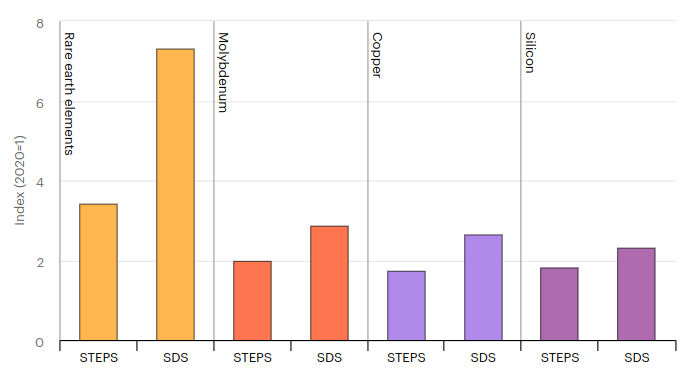
\includegraphics[width=\textwidth]{130quantification/external/energy_change_demand.png}
    \caption{Change in demand for selected elements}\label{fig:energy_change_demand}
\end{figure}

\begin{figure}[h!]
    \centering
    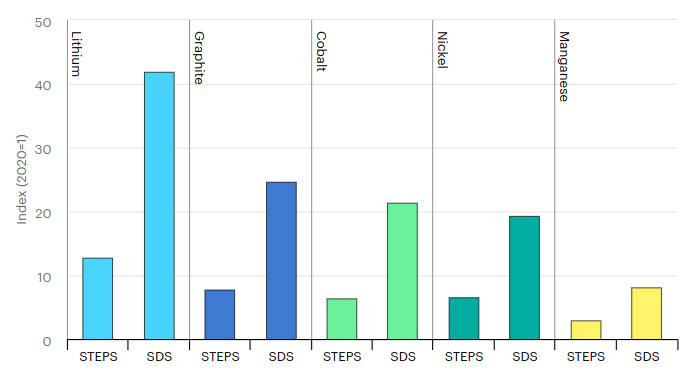
\includegraphics[width=\textwidth]{130quantification/external/energy_change_batt_demand.png}
    \caption{Change in demand for battery relevant elements}\label{fig:energy_demand_batt}
\end{figure}

\begin{figure}[h!]
    \centering
    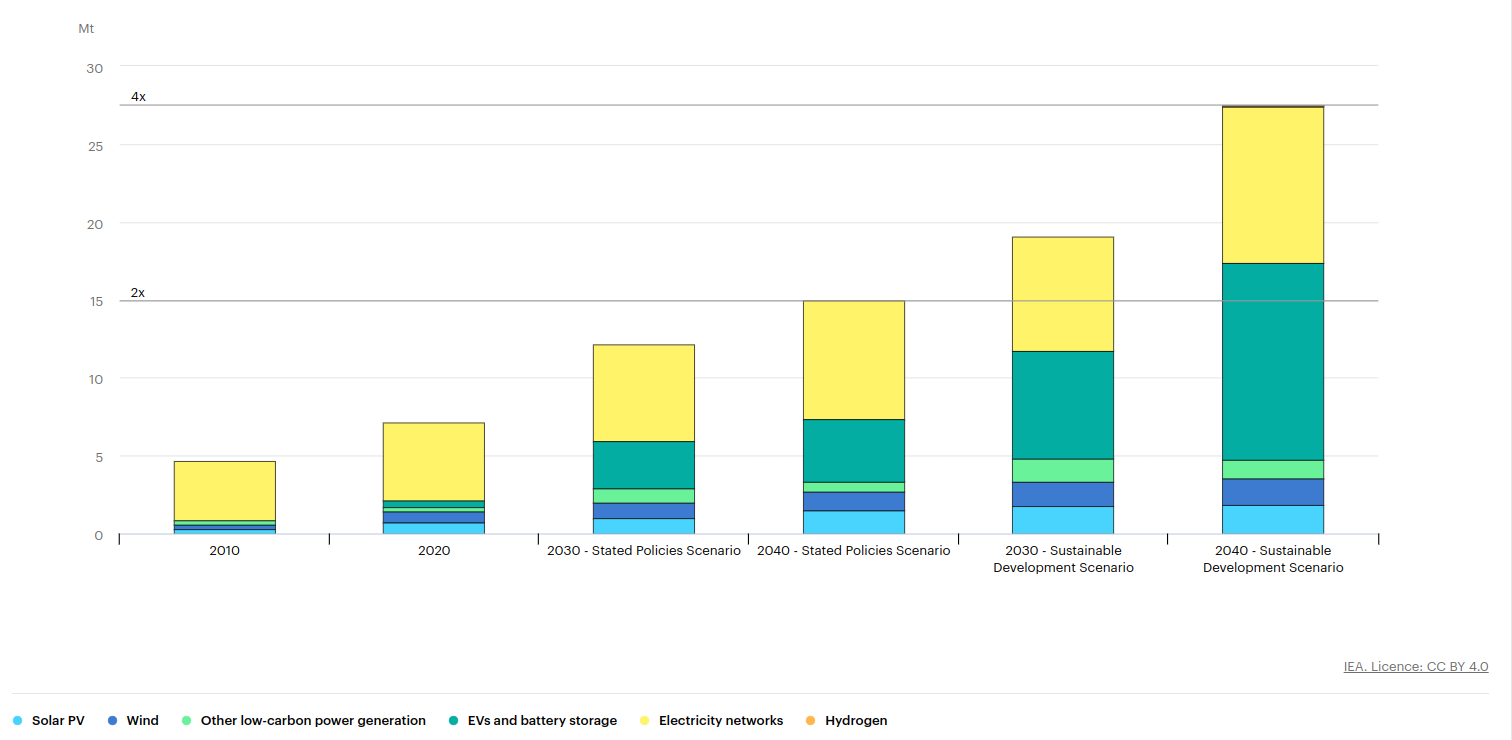
\includegraphics[width=\textwidth]{130quantification/external/energy_total_demand.png}
    \caption{Global mineral demand (total) under various scenarios}\label{fig:energy_mineral_total}
\end{figure}

\subsectionEndline
\clearpage

\subsubsection{Incorporation of the energy transition into individual waste stream models}


\boxws{This section will be filled out with the details of exactly how this parameter is incorporated into your stock and flow models}


\wasteSubsubsubsecBATT
\vspace{-1cm}
\begin{itemize}
    \item X
\end{itemize}

\wasteSubsubsubsecCDW
\vspace{-1cm}
\begin{itemize}
    \item X
\end{itemize}

\wasteSubsubsubsecELV
\vspace{-1cm}
\begin{itemize}
    \item X
\end{itemize}

\wasteSubsubsubsecMIN
\vspace{-1cm}
\begin{itemize}
    \item X
\end{itemize}

\wasteSubsubsubsecSLASH
\vspace{-1cm}
\begin{itemize}
    \item X
\end{itemize}

\wasteSubsubsubsecWEEE
\vspace{-1cm}
\begin{itemize}
    \item X
\end{itemize}



\subsectionEndline

\clearpage

\clearpage
\subsection{Supply constraints and market dynamics}

\boxreview{The precise methodology to be applied to determine the effects of hypothetical supply constraints and market dynamics on the model's outcomes has not yet been determined. This will be developed once the precise structure of the model has been finalised.}

\subsubsection{Introduction}

Supply constraints refer to limitations in the availability of resources that can impact industries and markets. These constraints can arise from various sources, such as natural resource depletion, geopolitical issues, economic factors, or environmental regulations. In the context of waste generation, collection, and recovery, supply constraints can significantly affect the dynamics of the entire system.

Market dynamics refer to the interactions between supply and demand that determine the prices of goods and services. These dynamics are influenced by various factors, such as the availability of resources, technological change, the state of the economy, and governmental policies.

Incorporating these economic factors into waste management models is essential to understand and predict the behavior of waste systems under different economic conditions. Accurate modeling can aid in making informed decisions regarding waste management policies and practices.

The following section details the importance of supply constraints and market dynamics and introduces the proposed strategy for incorporating these 'outside' elements in the modelling work in FutuRaM.


\subsubsection{Impacts of supply constraints and market dynamics}

\subsubsubsection{Impact on Waste Generation}
Constraints on the supply of materials can lead to alterations in waste composition. For instance, scarcity in a particular raw material can decrease the production and subsequent waste of products made from that material.

\subsubsubsection{Impact on Collection and Recovery Systems}
The availability of resources dictates the priorities of waste collection and recovery systems. Material scarcity can shift the focus towards recycling, while abundance might lead to alternative materials being preferred.

\subsubsubsection{Lag Times to Recovery}
The scarcity of materials can extend the time products remain in use before entering the waste stream, affecting the timing and efficiency of waste recovery systems.

\subsubsection{Economic Factors Influencing Waste Management}
Economic aspects like prices, subsidies, and taxation play a crucial role in waste management, especially in the context of supply constraints.

\subsubsubsection{Influence of Raw Material Prices}
High prices for primary raw materials can incentivize the recycling of secondary materials. This economic motivation can lead to advancements in recycling technology and increased recycling efforts.

\subsubsubsection{Secondary Raw Material Pricing}
The pricing of secondary raw materials, often influenced by the availability and price of primary materials, affects their attractiveness for recycling. Competitive pricing of secondary materials can promote their use over primary materials.

\subsubsubsection{Governmental Policies: Subsidies and Taxation}
Policies involving subsidies for recycling activities or taxation on primary raw materials can shape the waste management landscape. These fiscal tools can encourage or discourage recycling based on their design and application.

\subsubsubsection{Market Dynamics and Policy Interventions}
Market dynamics, influenced by policy interventions, can also impact waste management. For example, a policy promoting the use of recycled materials can alter market preferences and boost recycling efforts.

\subsubsection{Incorporation of supply constraints and market dynamics into the model}

\subsubsubsection{Sensitivity Analysis}

Sensitivity analysis is an instrumental approach in modelling to ascertain the impact of supply constraints and market dynamics on the waste management system. This technique involves systematically varying parameters within the model and observing the resultant effects on the output. It is particularly beneficial in identifying which variables have the most significant influence on the system's behaviour. 


Global Sensitivity Analysis, an extension of this concept, examines the entire parameter space, offering a comprehensive view of potential model responses to changes in input factors. This method is crucial in revealing the relative importance of different variables and can highlight areas where the system is most susceptible to economic fluctuations. 


By utilising sensitivity analysis, decision-makers can better understand the robustness of their systems and formulate strategies that are resilient to economic uncertainties.

\boxgreen{EXAMPLE}{
\textbf{Impact of Raw Material Prices and Government Subsidies on Recovery System:}
\begin{description}
    \item[Scenario:] The model tests scenarios with significant fluctuations in raw material prices. In certain scenarios, a government subsidy is introduced to set a minimum price for recycled materials, ensuring their economic viability.
    \item[Analysis:] Sensitivity analysis evaluates the effect of raw material price changes on the profitability and viability of the recovery system. It also tests the impact of government subsidies in stabilising the system against these fluctuations.
    \item[Outcome:] This analysis can reveal the dependency of recovery operations on raw material market prices and the effectiveness of government subsidies in mitigating associated risks.
\end{description}
}

\boxgreen{EXAMPLE}{
\textbf{Reduction of a Valuable Material in the Waste Stream:}
\begin{description}
    \item[Scenario:] The model explores a situation where a previously abundant and valuable material becomes scarce in the waste stream.
    \item[Analysis:] This sensitivity analysis investigates the impact of reduced availability of this valuable material on the overall profitability of the waste management system.
    \item[Outcome:] It identifies critical thresholds where a reduction in material significantly affects the system's financial viability, guiding strategies for diversifying material recovery or exploring alternative revenue sources.
\end{description}
}

\subsubsubsection{Optimisation}

Optimisation techniques are employed to identify the most efficient operational settings for the waste management system under diverse economic conditions. By modelling various local scenarios that encapsulate different economic realities –-- such as varying levels of resource scarcity, price dynamics of primary versus secondary materials, and the impact of subsidies or taxes –-- the model aims to find the optimal balance. This balance could be in terms of cost-effectiveness, resource utilization, environmental impact, or a combination of these factors. Optimization provides a framework to make data-driven decisions that can enhance the efficiency and sustainability of the waste management system.

Multi-Objective Optimisation is a key aspect of this process, where multiple conflicting objectives are considered simultaneously. This approach is essential in waste management systems, where there is often a need to balance economic goals with environmental sustainability. 

By employing optimisation techniques, particularly Multi-Objective Optimisation, the model can provide insights into the trade-offs and synergies between different objectives, thereby facilitating more informed and balanced decision-making in waste management policies and operations.

\boxgreen{EXAMPLE}{
\textbf{Responding to Sudden Demand Increase for a Previously Less Valuable Material (Element X):}
\begin{description}
    \item[Scenario:] The model simulates a sudden increase in demand and price for a specific material (Element X) that was previously less valuable.
    \item[Analysis:] The system's response is optimized to maximise profitability under this new market condition, involving adjustments in collection and processing priorities towards Element X.
    \item[Outcome:] The optimisation indicates the most effective strategies for reallocating resources and operations to capitalise on the increased demand for Element X, enhancing profitability.
\end{description}
}

\boxgreen{EXAMPLE}{
\textbf{Optimizing for Environmental and Economic Goals amid Rising Carbon Emission Costs:}
\begin{description}
    \item[Scenario:] The model considers a significant increase in the cost of carbon emissions, impacting the expense of recovery operations.
    \item[Analysis:] The optimisation aims to balance environmental impact (carbon footprint) with economic viability, exploring operational adjustments like adopting more carbon-efficient recovery processes or prioritising materials with higher primary carbon footprints (offsets and substitution).
    \item[Outcome:] This approach yields insights into effective strategies for maintaining profitability while minimising environmental impact, aiding the system in achieving a dual bottom line of environmental sustainability and financial health.
\end{description}
}

\subsectionEndline

\clearpage

\subsubsection{Relevance of supply constraints and market dynamics for FutuRaM's waste streams}

\wasteSubsubsubsecBATT
\begin{itemize}
    \item Fluctuating availability and prices of lithium and cobalt can significantly impact the recycling value and processes for batteries.
    \item Governmental policies on battery disposal and recycling can alter the landscape of battery waste management, influencing recycling rates and methodologies.
\end{itemize}

\wasteSubsubsubsecCDW
\begin{itemize}
    \item Variations in the construction market and raw material prices can influence the generation and composition of construction and demolition waste.
    \item Economic incentives and regulatory frameworks for sustainable construction practices can drive the recycling and reuse rates of CDW.
\end{itemize}

\wasteSubsubsubsecELV
\begin{itemize}
    \item Changes in the metal market, particularly for steel and aluminium, can impact the profitability of recycling ELVs.
    \item Environmental regulations on vehicle disposal and recycling can shape the recovery strategies for ELV waste.
\end{itemize}

\wasteSubsubsubsecMIN
\begin{itemize}
    \item Market demand for specific minerals can influence the focus and intensity of recovery efforts from mining residues.
    \item Policy changes regarding mine waste management can lead to shifts in recovery and disposal practices for mining residues.
\end{itemize}

\wasteSubsubsubsecSLASH
\begin{itemize}
    \item The variability in the composition of slags and ashes due to different industrial processes and raw materials can significantly influence recovery and recycling strategies.
    \item Market conditions for secondary raw materials derived from slags and ashes, such as metals, can greatly affect the economic viability of their recovery and recycling processes.
\end{itemize}

\wasteSubsubsubsecWEEE
\begin{itemize}
    \item Fluctuations in precious metal prices can affect the economics of recycling electronic waste.
    \item Evolving technology and product lifecycles can influence the generation and composition of WEEE, affecting recycling strategies.
\end{itemize}

\subsectionEndline


\clearpage
\subsubsection{Incorporation of supply constraints and market dynamics into individual waste stream models}

\boxws{This section will be filled out with the details of exactly how this parameter is incorporated into your stock and flow models}

\wasteSubsubsubsecBATT
\begin{itemize}
    \item X
\end{itemize}

\wasteSubsubsubsecCDW
\begin{itemize}
    \item X
\end{itemize}

\wasteSubsubsubsecELV
\begin{itemize}
    \item X
\end{itemize}

\wasteSubsubsubsecMIN
\begin{itemize}
    \item X
\end{itemize}

\wasteSubsubsubsecSLASH
\begin{itemize}
    \item X
\end{itemize}

\wasteSubsubsubsecWEEE
\begin{itemize}
    \item X
\end{itemize}


\subsectionEndline

\clearpage

% \clearpage
% \input{132e-quantification_external_supply}
\clearpage

\subsection{Conclusion}

\boxreview{This conclusion will be compiled once the individual waste stream sections for each parameter are complete.}